\begin{tikzpicture}[scale=0.7, transform shape]
	\onslide<2->{

		\draw[draw=green!50,fill=green!10,thick,solid,rounded corners] (3.4,0.6) rectangle (0.6,3.4);

		\node[inner sep=0pt] (D) at (2,2)
		{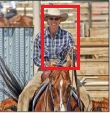
\includegraphics[scale=0.8]{images/cowboy_pred.jpg}};
		\draw [draw=yellow,fill=yellow] (2.15,2.4) circle (0.06);    
		\node[yellow] at (2.15,2.2) {($x$,$y$)};     
		\node[yellow] at (2,1.5) {$w$};
		\node[yellow] at (1.5,2.4) {$h$};
		\node at (2,0) {Proposed Box};
	}
	
	\onslide<3->{
		\draw[draw=green!50,fill=green!10,thick,solid,rounded corners] (7.4,0.6) rectangle (4.6,3.4);

		\node[inner sep=0pt] (E) at (6,2)
		{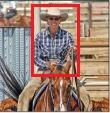
\includegraphics[scale=0.8]{images/cowboy_true.jpg}}; 
		\node[yellow] at (6,1.4) {$w^*$};     
		\node[yellow] at (5.4,2.4) {$h^*$};
		\draw [draw=yellow,fill=yellow] (6.1,2.4) circle (0.06);    
		
		\node[yellow] at (6.1,2.2) {($x^*$,$y^*$)};     
		\node at (6,0) {True Box};
	}
	
	\onslide<6->{\node at (4.1,-0.6) {z : features from pool5 layer of the network};
	}
\end{tikzpicture}
